% ----------------------------------------------------------
\chapter{Desenvolvimento}
% ----------------------------------------------------------

% ----------------------------------------------------------
\section{Aplicativo web}
% ----------------------------------------------------------

O sistema do aplicativo tem como essência três partes, comentadas abaixo e ilustradas na \autoref{fig:proj-ideia}.

\begin{itemize} 
	\item \textbf{Funcionalidade:} a função básica do aplicativo é possibilitar que uma \textbf{Empresa B}, consumidora de resíduos (matéria-prima), localize uma \textbf{Empresa A}, geradora de resíduos, afim de que haja, de alguma forma, uma comuta entre as partes;
	\item \textbf{Pontuação (\textit{Score}):} para alcançar a funcionalidade é necessário definir métricas que decidam quando uma \textbf{Empresa A} é melhor candidata a fornecer resíduos do que uma \textbf{Empresa C}. Essas métricas são consolidadas em uma pontuação ou score; 
	\item \textbf{Fontes de Dados:} para obtenção das métricas, necessitam-se de bases de dados com a capacidade de fornecer os dados que se necessitam de forma prática, confiável, com facilidade de manuseio e baixo custo.
\end{itemize}

\begin{figure}[htb]
	\caption{\label{fig:proj-ideia} Esquema do projeto do aplicativo web}
	\begin{center}
		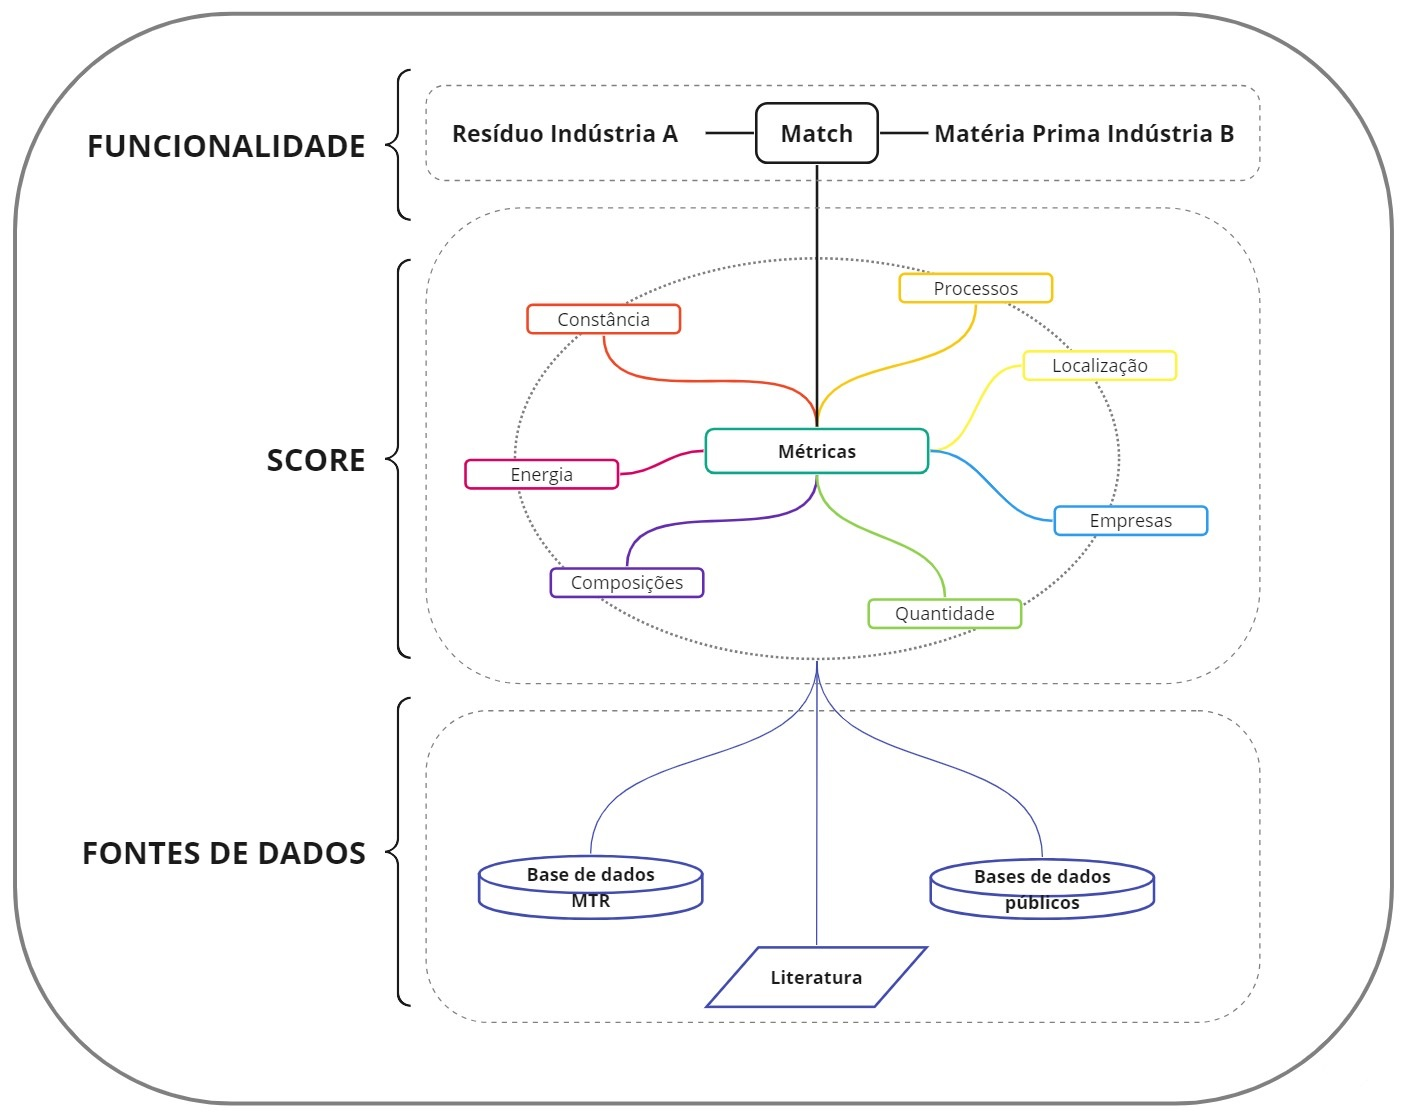
\includegraphics[scale=0.48]{images/TCC Board.jpg}
	\end{center}
	\fonte{Elaborado pelo Autor (2023)}
\end{figure}

As fontes de dados foram citadas na \autoref{section:Fontes} e neste capítulo na \autoref{section:consolida}. A funcionalidade (Conceito) e as métricas serão mencionadas nas seções a seguir.


% ----------------------------------------------------------
\subsection{Público-alvo}
% ----------------------------------------------------------

Com esse aplicativo, tem-se objetivo de alcançar tanto potenciais consumidores de matéria-prima quanto geradores de resíduo, uma vez que se entende que não existe apenas geradores ou consumidores numa economia circular. Esta dinâmica está representada na \autoref{fig:user-flux}, onde fixado um Usuário 1, este pode atuar como gerador para X Usuários ou consumidor de X Usuários.

\begin{figure}[htb]
	\caption{\label{fig:user-flux} Fluxo do usuário no app}
	\begin{center}
		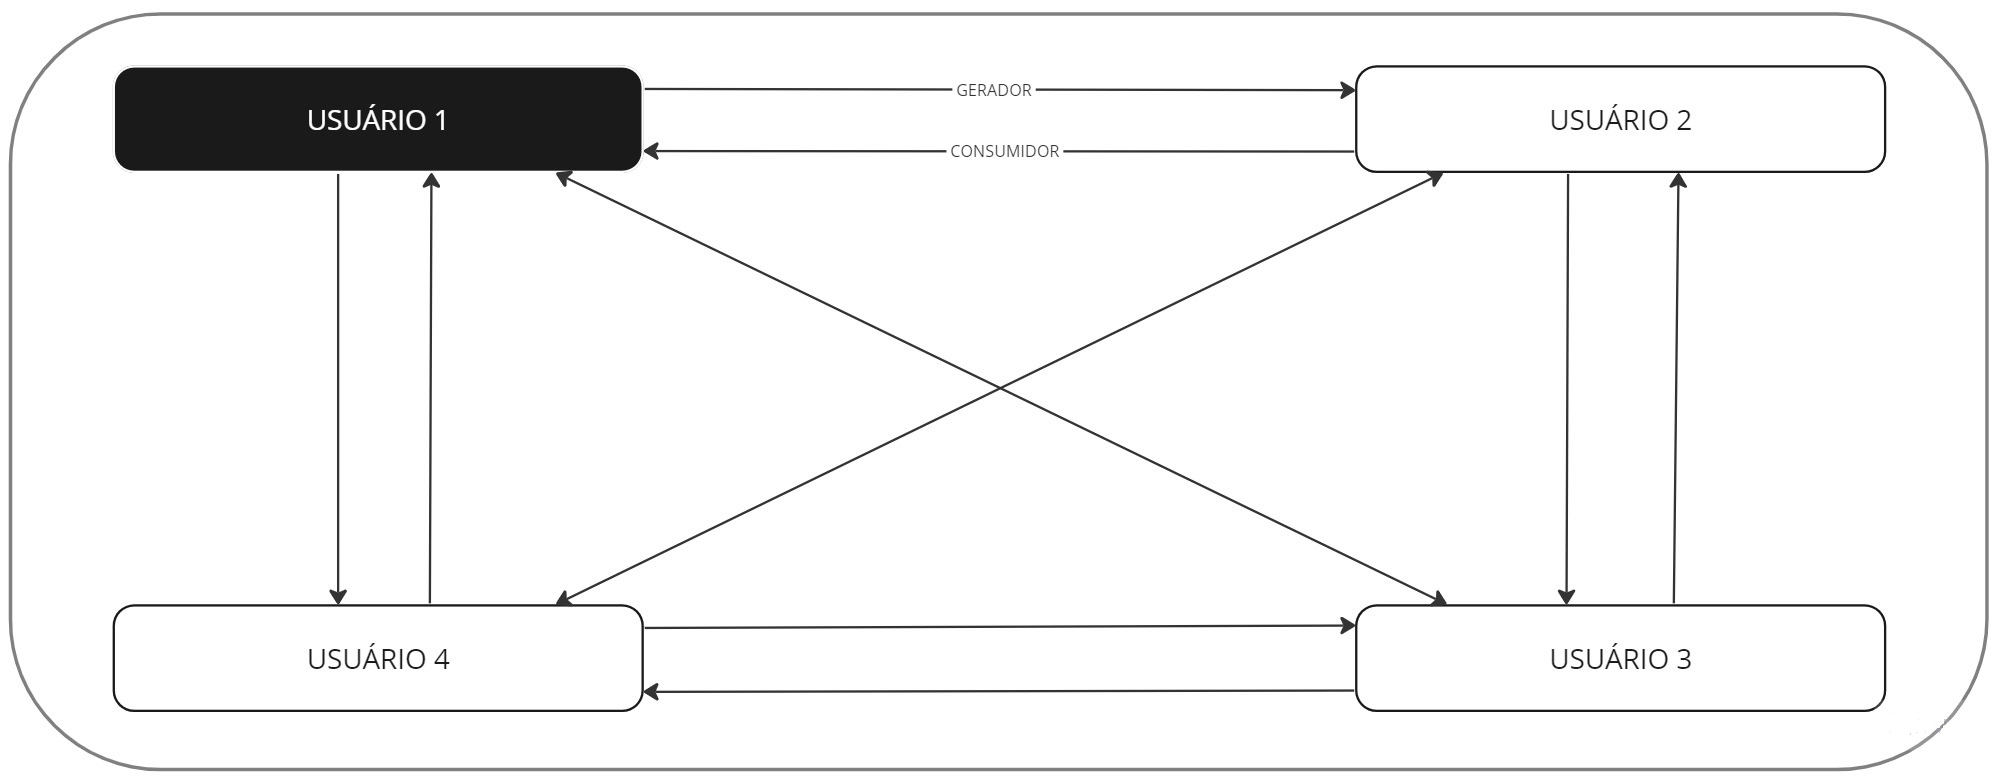
\includegraphics[scale=0.38]{images/user-flux.jpg}
	\end{center}
	\fonte{Elaborado pelo Autor (2023)}
\end{figure}

% ----------------------------------------------------------
\subsection{Conceito I}
% ----------------------------------------------------------

Visando amostrar a funcionalidade básica do sistema, esse foi o conceito prototipado e disponibilizado para teste, servindo de base também para o Conceito II. Nesse sentido, o aplicativo é composto por:

\begin{itemize} 
	\item \textbf{Página Inicial:} é a página de boas-vindas, deve conter uma breve explicação do funcionamento e contexto do aplicativo e ter uma estética moderna e atrativa;
	\item \textbf{Janela de Cadastro/Entrada:} entende-se necessário o cadastro, por mais simples que seja, para que se tenha estatísticas de uso do site. Os componentes básicos do cadastro são o e-mail e a senha; 
	\item \textbf{Janela de Aquisição/Aproveitamento:} com o cadastro, o usuário é direcionado à um painel com um menu que represente Consumo, nesta opção encontra-se um módulo “Localizador de Resíduo”. Nessa função está a janela de aquisição ou aproveitamento de resíduos que contém campos em forma de formulário que irão compor o score para a combinação do usuário com outras empresas, neste caso, o Capítulo, Subcapítulo e Código do \gls{IBAMA}, o Município do usuário/empresa e a Quantidade de resíduo desejada;
	\item \textbf{Janela de resultado} após envio do formulário, segue-se para a janela de resultados, que apresenta uma classificação (\textit{“ranking”}), em forma de lista, da combinação mais recomendada para a menos recomendada com base na pontuação.
\end{itemize}

Na \autoref{fig:app-flux1} é possível visualizar os itens mencionados na forma de fluxograma, contudo vale ressaltar que se trata de uma visão genérica e pode diferir do protótipo existente.

\begin{figure}[htb]
	\caption{\label{fig:app-flux1} Fluxo do aplicativo - Conceito I}
	\begin{center}
		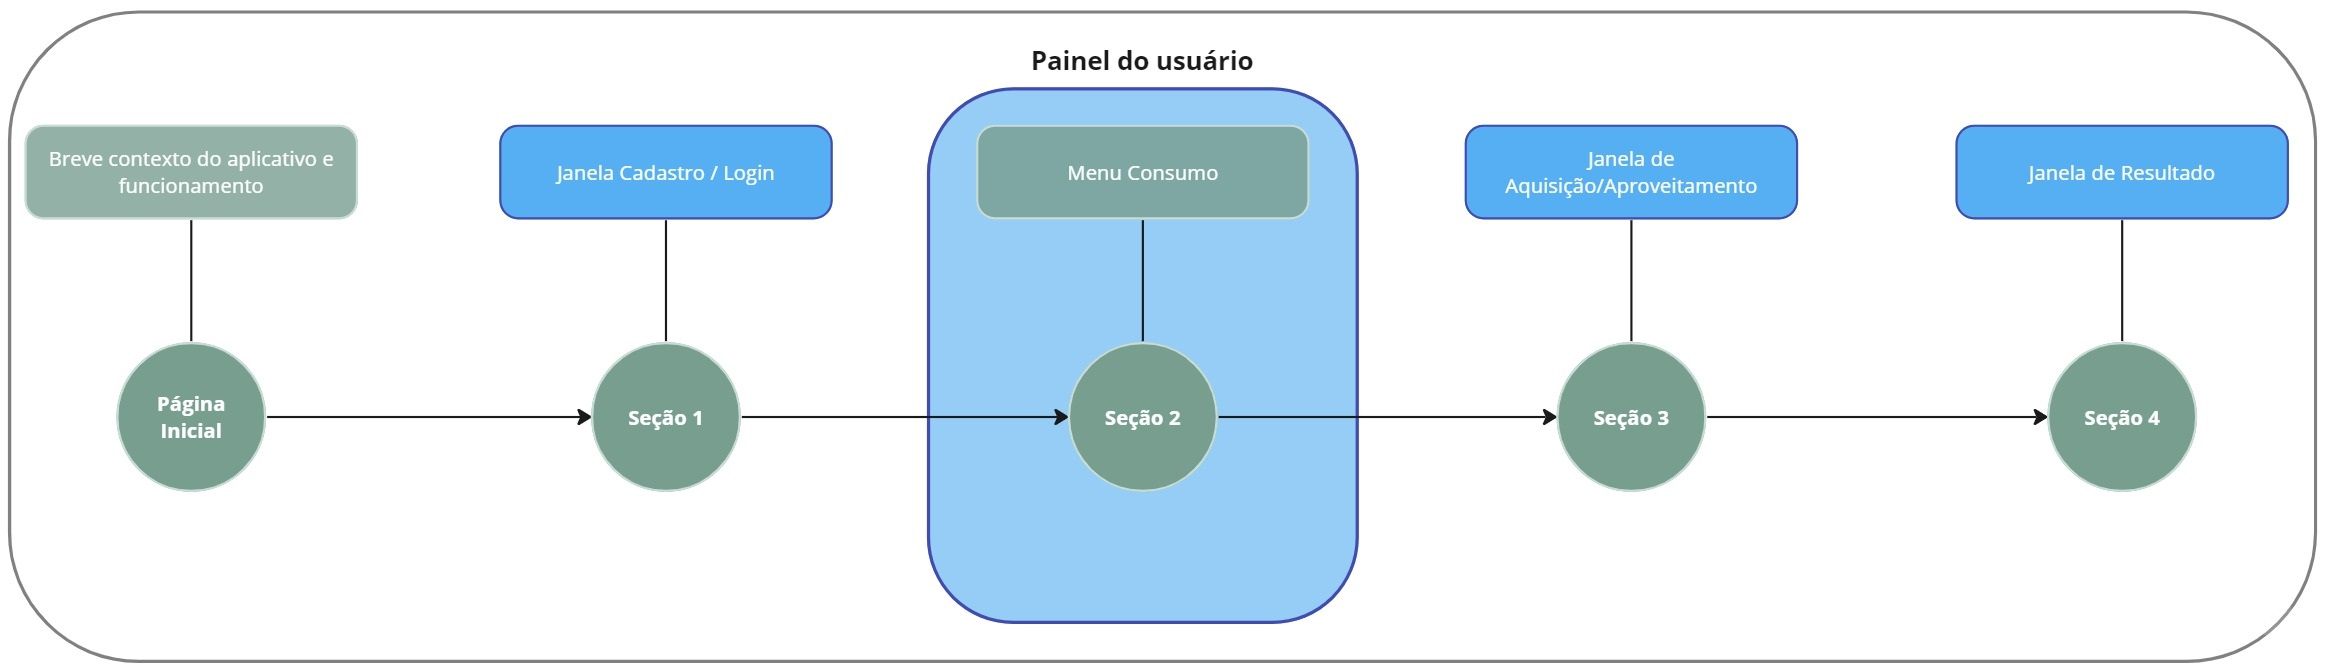
\includegraphics[scale=0.33]{images/app-flux1.jpg}
	\end{center}
	\fonte{Elaborado pelo Autor (2023)}
\end{figure}

% ----------------------------------------------------------
\subsection{Conceito II}
% ----------------------------------------------------------

Numa versão mais completa do aplicativo, adiciona-se ao Conceito I, os menus Geração e Chat, além disso, propõe-se uma abordagem para a janela de aquisição que abrange também usuários sem conhecimento prévio do resíduo, mas que entendem bem as etapas dos processos dentro da indústria. Na \autoref{fig:app-flux2} está ilustrado em formato de fluxograma as adições ao Conceito I.

Sabendo que a comunicação é essencial para qualquer comuta entre os usuários, adiciona-se o recurso de \textbf{Chat}, a qual facilitaria o contato entre empresas geradoras e consumidoras cadastradas. Nesse caminho, entende-se que o aplicativo deixa de se voltar apenas ao consumo, mas também à geração, e em vista disso é adicionado o menu \textbf{Geração}, o qual abarca as janelas de \textbf{Gerenciamento} e \textbf{Destinação}, a primeira possibilitaria a empresa gerenciar os resíduos sólidos, organizando as etapas de geração, armazenamento, transporte e destinação; seria possível também automatizar a geração de \gls{MTR}s através de integrações por \gls{API}, como a disponibilizada pelo \textcite{cetesb_web_2021}; a segunda janela, utiliza-se pelo usuário que deseja destinar ou ofertar o resíduo para outra empresa, seguindo a mesma dinâmica do menu de consumo

\begin{figure}[htb]
	\caption{\label{fig:app-flux2} Fluxo do Aplicativo - Conceito II}
	\begin{center}
		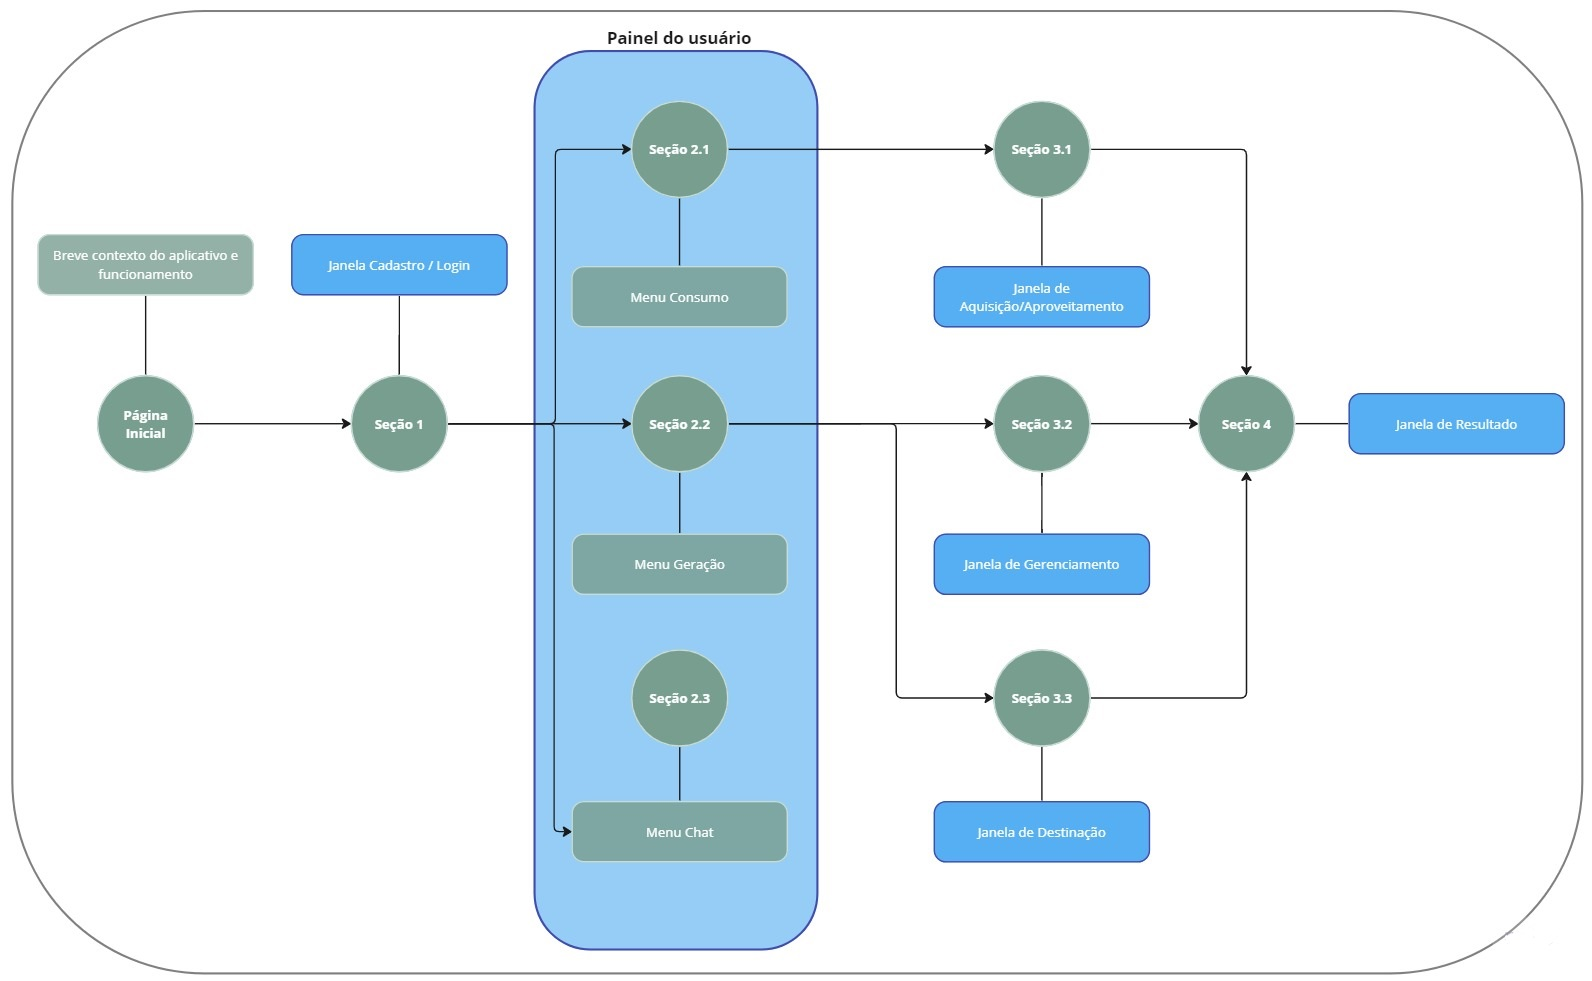
\includegraphics[scale=0.46]{images/app-flux2.jpg}
	\end{center}
	\fonte{Elaborado pelo Autor (2023)}
\end{figure}

A respeito do consumo, para justificar a mudança de abordagem, vale-se citar como exemplo a dissertação de \textcite{lima_jose_2002}, que discute a utilização da lama gerada pela etapa de lavagem do processo de extração de minério de ferro como complemento à argila da massa de placas cerâmicas. 

Nesse cenário, para a Empresa A da indústria de fabricação de revestimento cerâmico, sem conhecimento que esse resíduo pode ter valor, apresenta-se um módulo de “Combinação por fluxo”, em que a empresa seleciona o ramo da indústria (Cerâmica) e o processo deste ramo que deseja navegar (Fabricação de Revestimento Cerâmico), abre-se então um painel com um fluxo simplificado do processo selecionado\footnote{Várias etapas do processo de Fabricação de revestimento cerâmico foram omitidas, como a atomização, secagem e esmaltação, além disso, sabe-se que o fluxo não é linear.}  indicando as entradas e saídas de cada etapa, conforme ilustrado na \autoref{fig:revs-ceramico}. Ao selecionar o componente da etapa que se interessa (Argila) é exibido um painel com possíveis resíduos que podem complementar ou substituir o componente selecionado. 

\begin{figure}[htb]
	\caption{\label{fig:revs-ceramico} Fluxograma simplificado do processo de fabricação de revestimento cerâmico}
	\begin{center}
		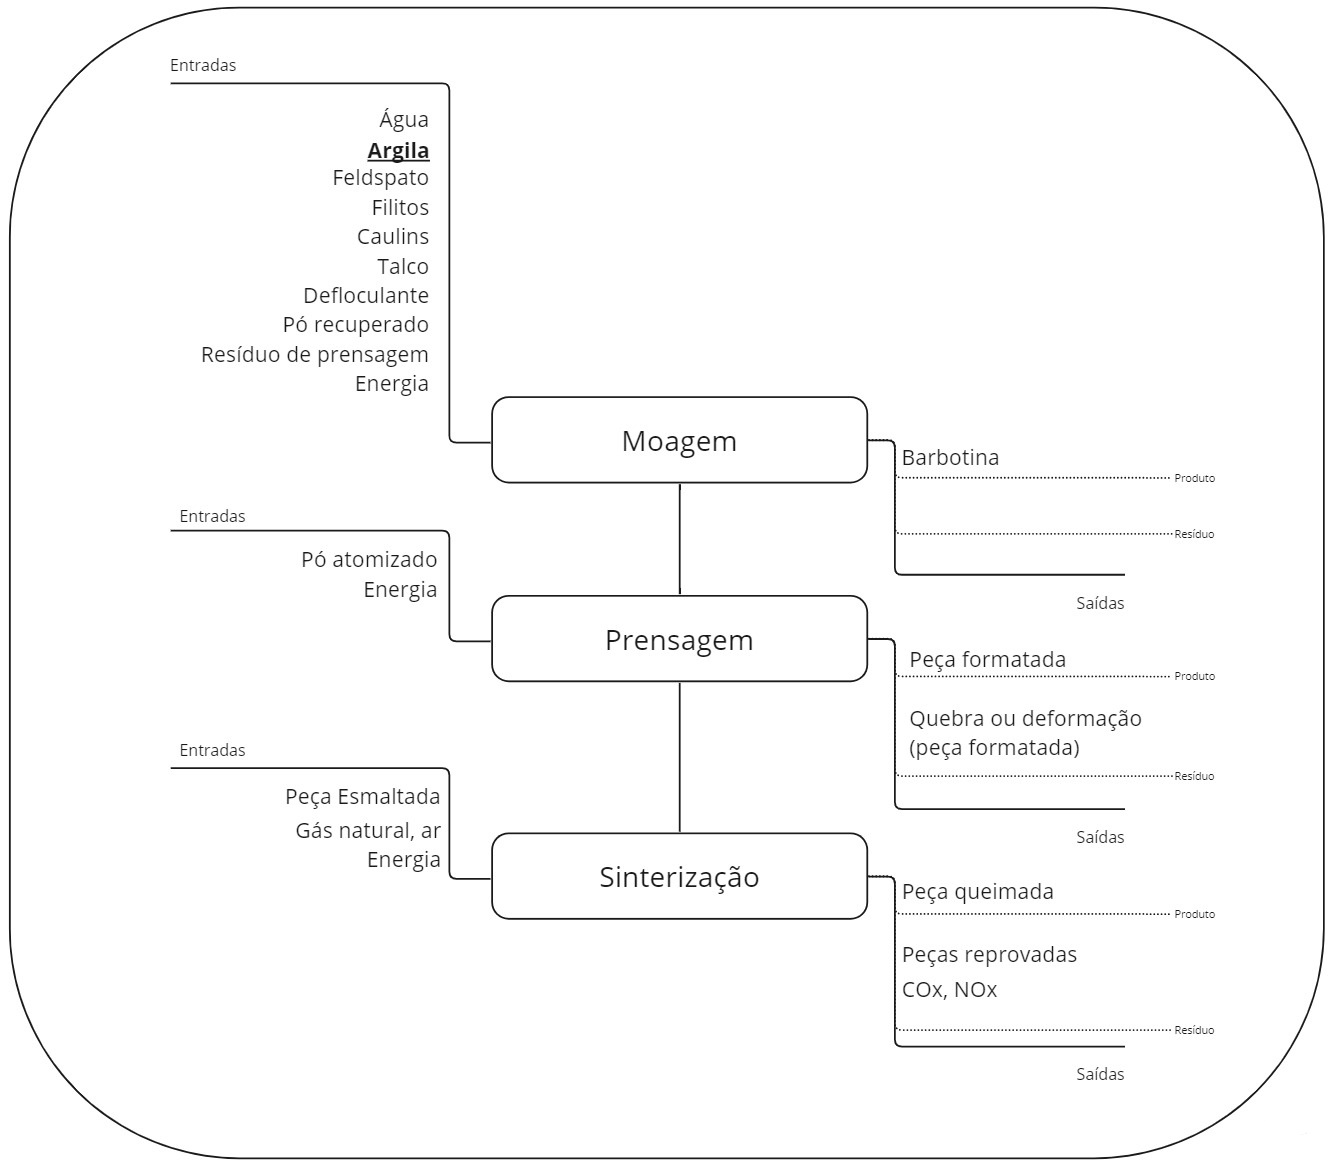
\includegraphics[scale=0.46]{images/revs-ceramico.jpg}
	\end{center}
	\fonte{Elaborado pelo Autor (2023)}
\end{figure}

O painel de resíduos é a fase a mais importante e desafiadora do ponto de vista técnico, para prover as opções de resíduos, faz-se necessário uma busca em artigos, dissertações, teses por estudos de utilização de resíduos em processos industriais. Na visão deste trabalho, sugere-se o treinamento de um \gls{LLM} com uma base de trabalhos acadêmicos direcionado ao tema, diga-se uma \gls{IA} de Ciência de Materiais ou utilização de \gls{IA}s existentes com foco em ciência, como a \textbf{Galactica} \cite{taylor_galactica_2022}. Outro ponto, é que até o momento da pesquisa realizada, a maioria dos trabalhos relacionados ao aproveitamento de resíduos sólidos no Brasil sequer mencionam uma classificação de resíduos, logo também seria necessário classificar o resíduo em estudo de acordo com a lista de resíduos do \gls{IBAMA}

No contexto, ao prosseguir com a seleção do resíduo seriam preenchidos os dados relativos à quantidade desejada e a localização da empresa, finalizando com os resultados da mesma forma que no Conceito I. Na \autoref{fig:app-mod2} estão representados os módulos da janela de aquisição que compõe o Conceito II.

\begin{figure}[htb]
	\caption{\label{fig:app-mod2} Fluxograma da janela de aquisição com a adição do módulo de “Combinação por fluxo”}
	\begin{center}
		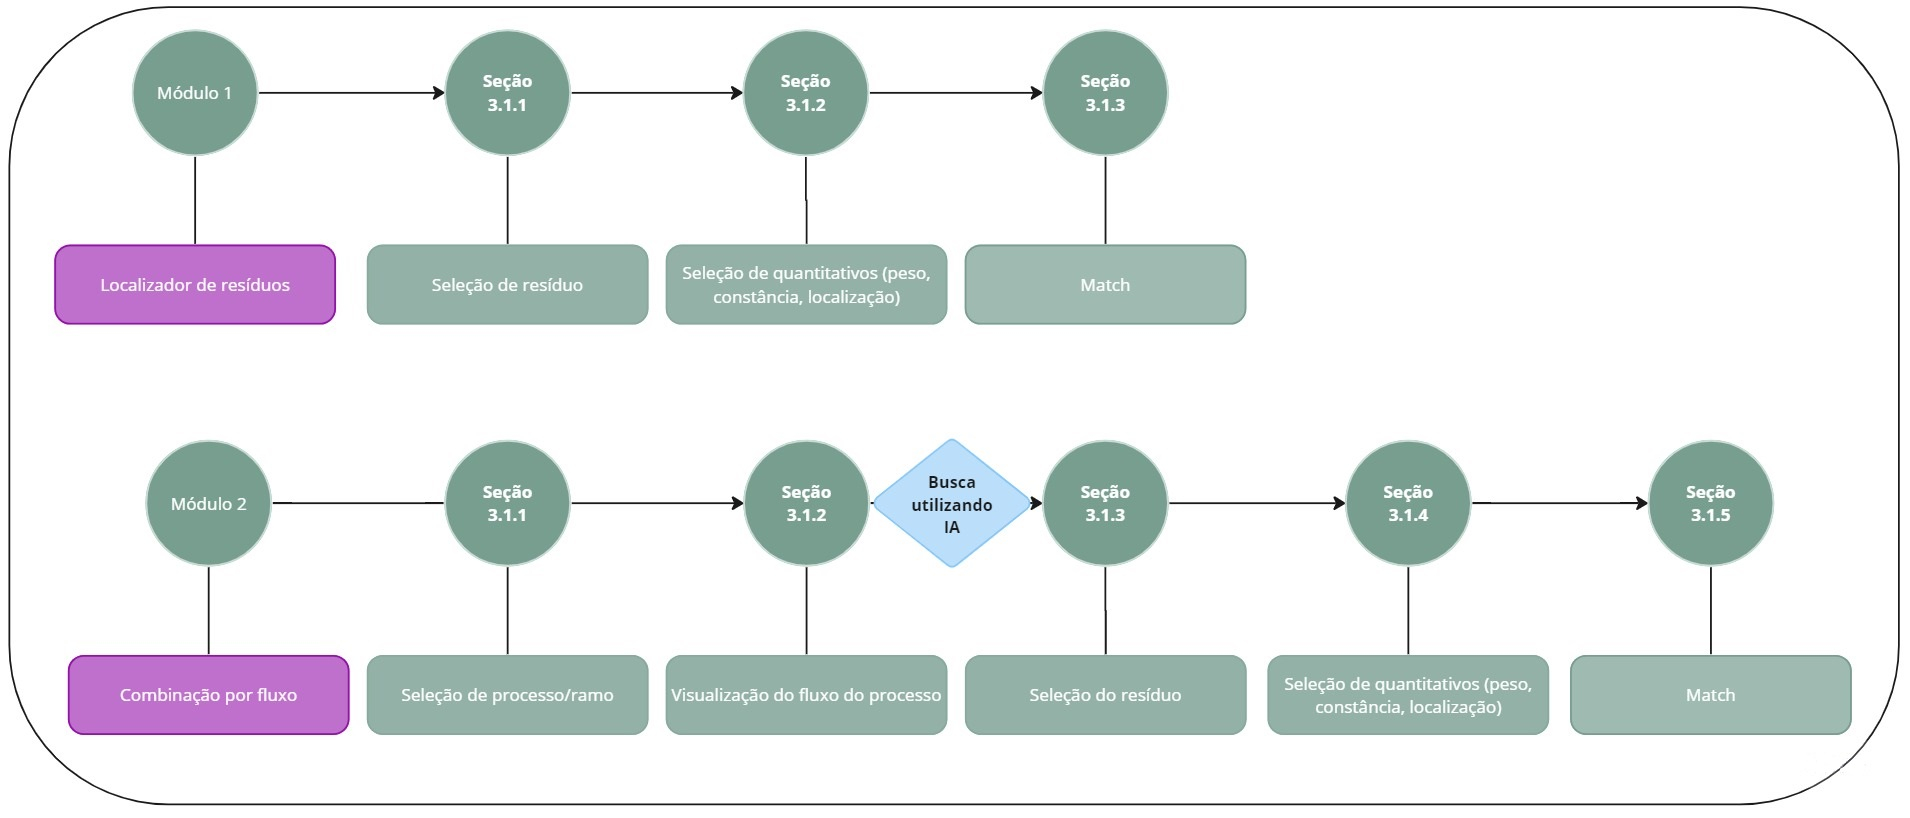
\includegraphics[scale=0.38]{images/app-mod2.jpg}
	\end{center}
	\fonte{Elaborado pelo Autor (2023)}
\end{figure}


% ----------------------------------------------------------
\subsection{Métricas para a combinação (\textit{“match”})}
% ----------------------------------------------------------

As métricas expostas aqui são variáveis que tentam aproximar a real necessidade das indústrias, para que os resultados da combinação estejam de acordo com as expectativas mínimas da empresa. Reconhece-se que existem mais parâmetros a se considerar, às vezes específicos para determinado processo de produção, porém na tentativa de generalizar foram comentadas as variáveis abaixo.

\begin{itemize} 
	\item \textbf{Distância:} fator que afeta a energia gasta para mover o resíduo do ponto A para o B, influenciando diretamente o custo da operação. Deve considerar a malha rodoviária ideal para o transporte, não apenas a menor distância;
	\item \textbf{Quantidade:} para inserir um resíduo numa etapa do processo, deve existir material suficiente para suprir as demandas de ambas as indústrias;
	\item \textbf{Constância:} a geração deve possuir uma frequência, de modo que seja possível um planejamento pela indústria consumidora de quanto em quanto tempo esse resíduo pode ser obtido;
  \item \textbf{Composição química:} é evidente que a consumidora preza por manter a qualidade dos produtos, e uma mudança de material base pode impactar negativamente se não forem conhecidas as substâncias que constituem o resíduo;
  \item \textbf{Estado:} para a consumidora conseguir utilizar o resíduo talvez sejam necessárias etapas de preparação, pois o resíduo pode estar em forma de cacos, pó, pellets, pasta etc. Isso também pode impactar a possibilidade de uso do resíduo.
\end{itemize}

Das métricas citadas, foram utilizadas para o protótipo apenas a Distância e a Quantidade, pois a Constância e o Estado são dados que não se conseguiu obter junto ao \gls{IMA/SC} devido a dificuldades no sistema interno, o primeiro depende de que os dados estejam em uma granularidade pelo menos mensal, o segundo é algo que consta nos \gls{MTR}s porém não foi incluso nos relatórios. A composição química não consta nos campos do \gls{MTR}, e por se tratarem de resíduos bastante específicos a cada ramo da indústria, pensa-se que seria preciso uma generalização com base na classificação do \gls{IBAMA}, o que é um desafio fora do escopo deste trabalho. 

% ----------------------------------------------------------
\subsection{Pontuação e estimativas para o resultado}
% ----------------------------------------------------------

Para os presentes cálculos, apenas as métricas de distância (\gls{d}) e quantidade são consideradas, tais grandezas estão diretamente relacionadas ao gasto de combustível para o transporte, o qual influencia tanto no custo quanto na pegada de carbono, ambos são estimados no resultado da combinação. No Brasil, em 2019, 64,9\% de toda a carga transportada no Brasil usou o sistema modal rodoviário \cite{cnt_o_nodate}, por essa razão esse foi o modo de transporte avaliado para esse trabalho.

Assumindo que o transporte do resíduo será feito através de um caminhão a diesel de até 16 \ensuremath{t}, segundo \textcite{bartholomeu_quantificacao_2006}, podemos definir as constantes:

\begin{itemize} 
	\item Fator de emissão de $CO_{2}$ do diesel: $2,7 kg CO_{2}/L $;
  \item Consumo médio de combustível: $ 3,4 \cdot 10^{-1} L/km $.
\end{itemize}

Assim, temos as variáveis: 

\begin{itemize} 
	\item Pegada de carbono (\gls{P}): 
  \begin{equation}\label{eq:Eq_1}
    \gls{P} = 9,2 \cdot 10^{-1} \cdot \gls{d} \hspace{10mm} (\ensuremath{kg} \hspace{1mm} CO_{2}/\ensuremath{km})
  \end{equation}
	\item Custo do transporte\footnote{Como exemplo, foi utilizado o preço médio do diesel S10 em Santa Catarina no mês de Novembro de 2023 ($R\$6,08/$\ensuremath{L}), contudo esse valor deve ser atualizado dinâmicamente no app.} (S): 
  \begin{equation}\label{eq:custo} 
    \gls{S} = 2,1 \cdot \gls{d} \hspace{5mm} (R\$/\ensuremath{km})
  \end{equation}  
\end{itemize}

Para o cálculo da pontuação será utilizada a equação abaixo, lendo-se que se a quantidade disponível (\gls{Q}) for 80\% inferior à solicitada pelo usuário  for 80\% superior à quantidade solicitada pelo usuário (\gls{q}), considera-se que a quantidade não terá impacto na pontuação.

\begin{equation}\label{eq:pont}
      \textbf{score} = 
  \begin{cases}
      \frac{q}{Q} \cdot \frac{10^2}{x^2 + 10^{-1}},& \text{se } \frac{q}{Q} \leq 0\,8\\
      \frac{10^2}{x^2 + 10^{-1}},              & \text{senão}
  \end{cases}
\end{equation}
\\
% ----------------------------------------------------------
\section{Protótipo}
% ----------------------------------------------------------

Como mencionado anteriormente, foi utilizado o Conceito I para elaboração do protótipo e para colocá-lo disponível na internet foi dado o nome de \textbf{“residuose”}, um jogo de palavras entre “resíduos” e “simbiose” para remeter ao tema central do sistema, que é fazer com que as empresas trabalhem em sinergia aproveitando os resíduos gerados entre si.

A previsão é que o website esteja online até Abril de 2024 no domínio url{https://residuose.tech}, contudo o cadastro de usuários será limitado, pois ainda não se tem a confirmação junto ao \gls{IMA/SC} para liberação dos dados de \gls{MTR}, como a razão social da empresa e o telefone, por exemplo. 

Na \autoref{fig:app-homepage} e \autoref{fig:app-logsign} estão ilustradas as páginas de entrada para o aplicativo, nota-se que o cadastro requer apenas o e-mail, o nome e uma senha.

\begin{figure}[H]
	\caption{\label{fig:app-homepage} Página inicial da aplicação}
	\begin{center}
		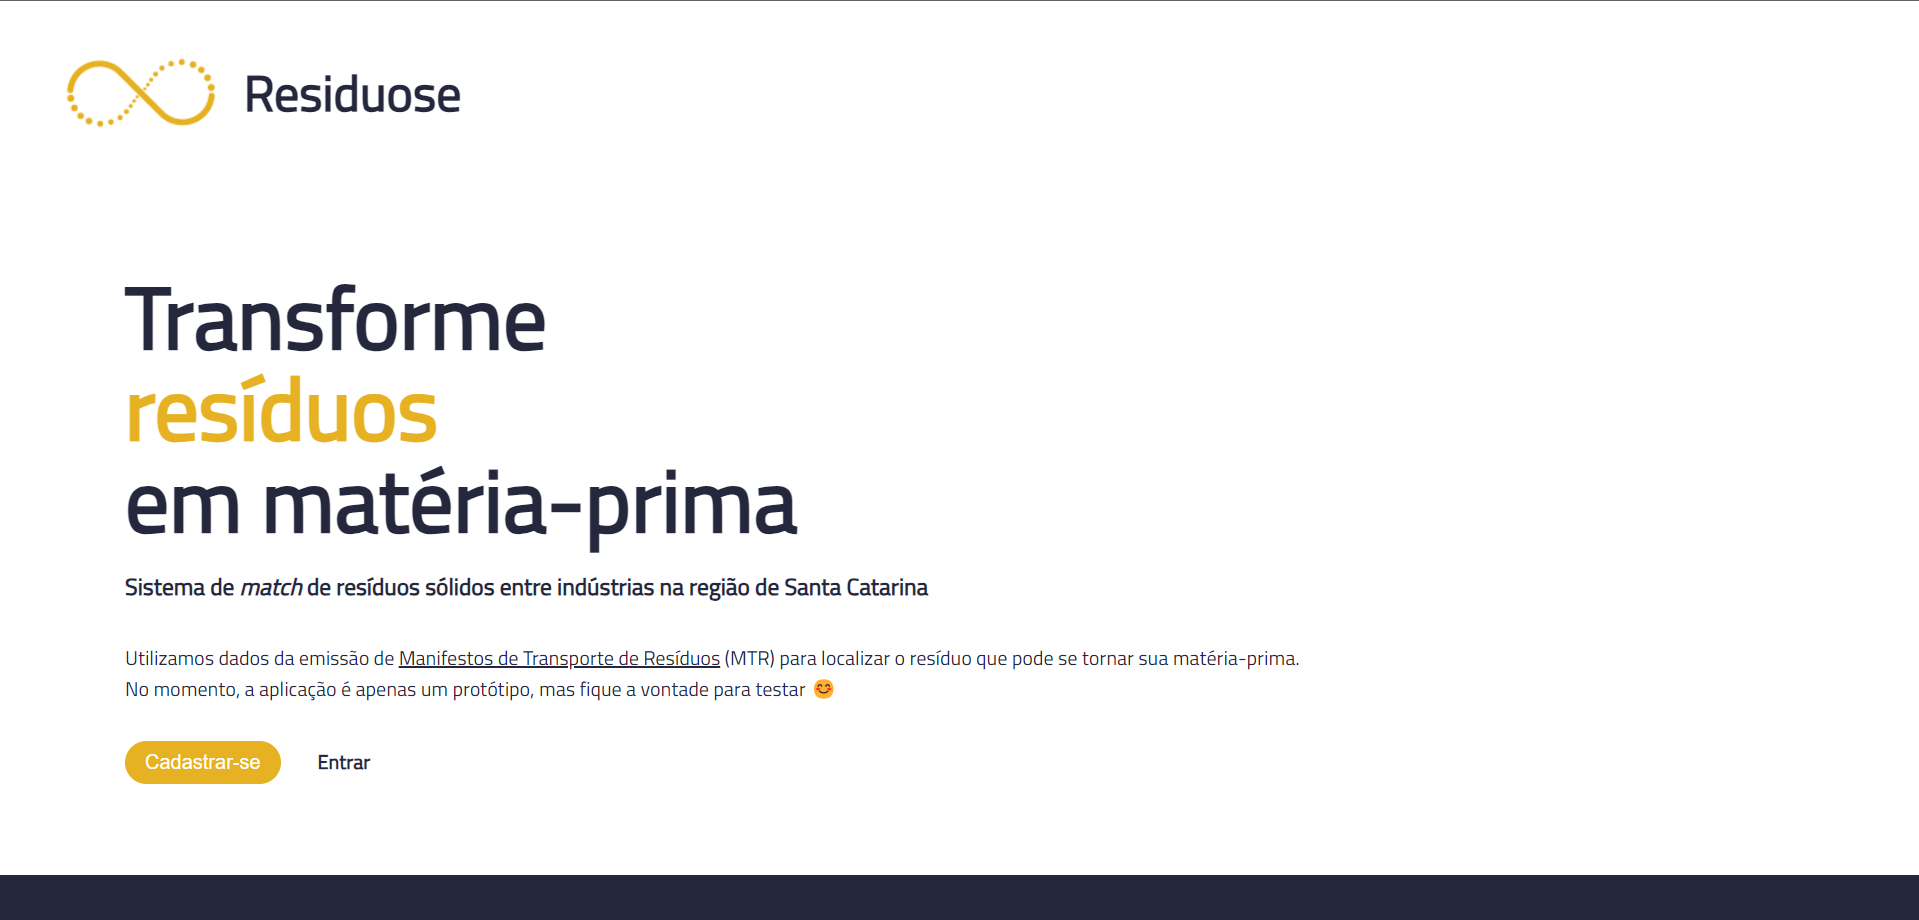
\includegraphics[scale=0.38]{images/homepage.png}
	\end{center}
	\fonte{Elaborado pelo Autor (2023)}
\end{figure}

\begin{figure}[H]
	\caption{\label{fig:app-logsign} Janelas de cadastro e entrada}
	\begin{center}
		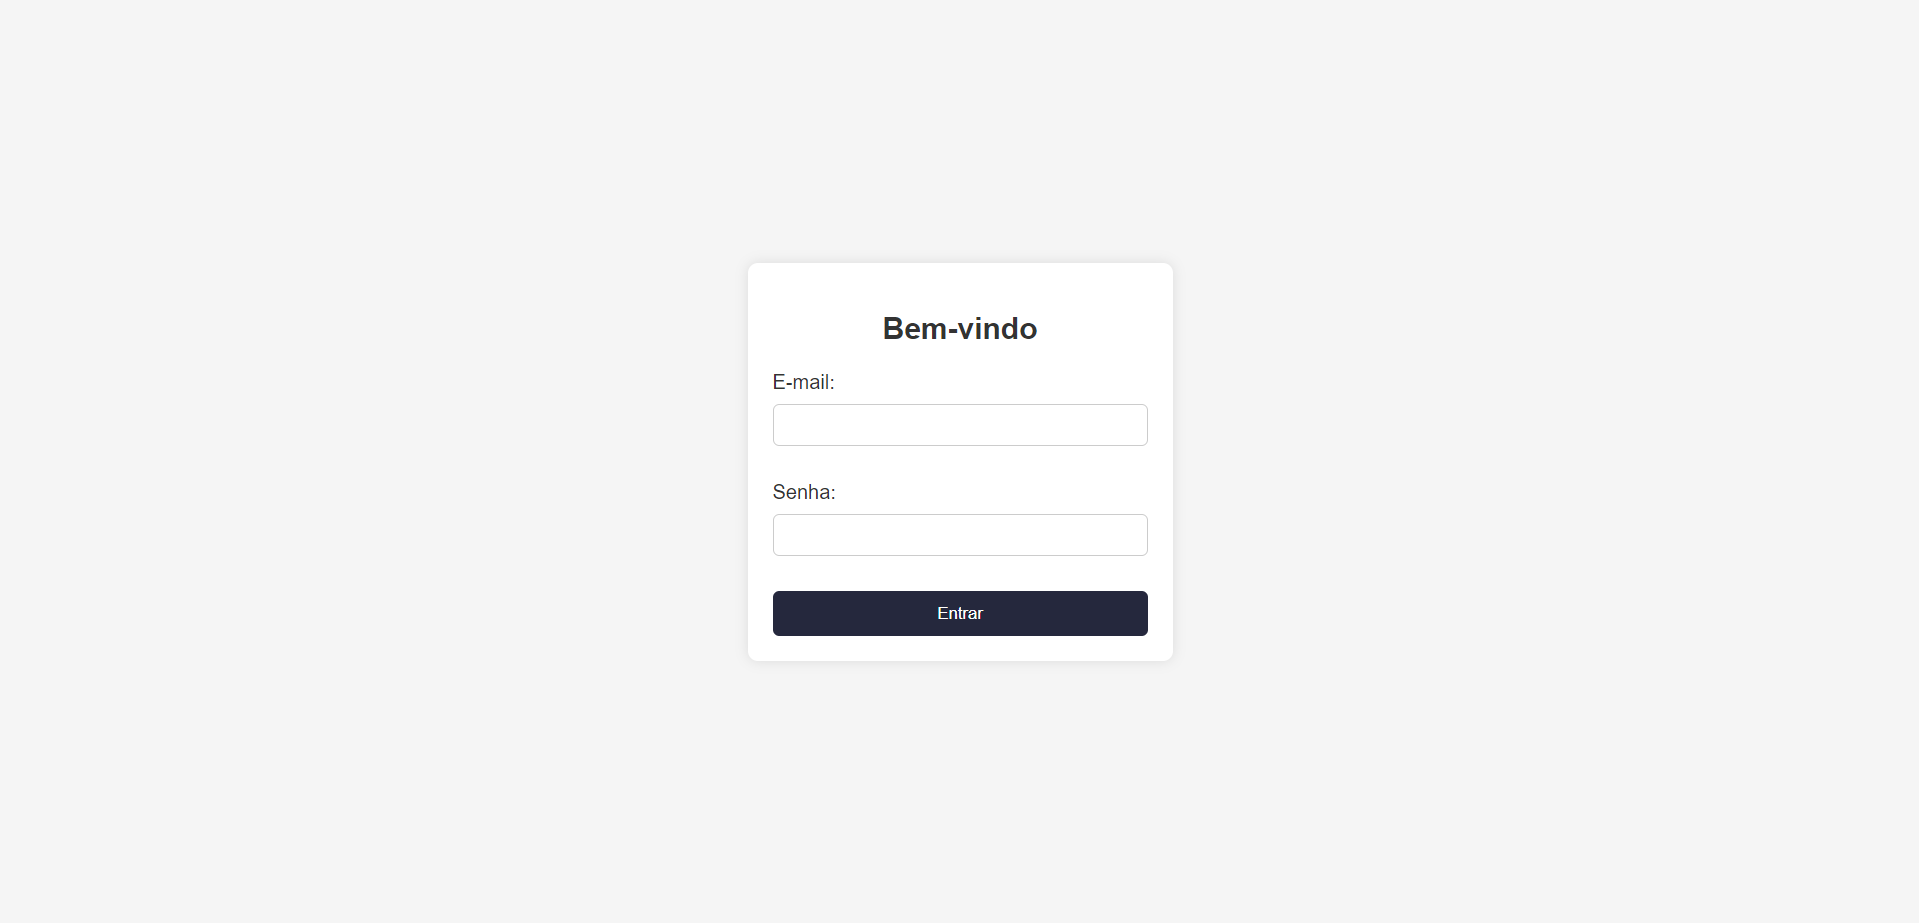
\includegraphics[scale=0.38]{images/entrar.png}
    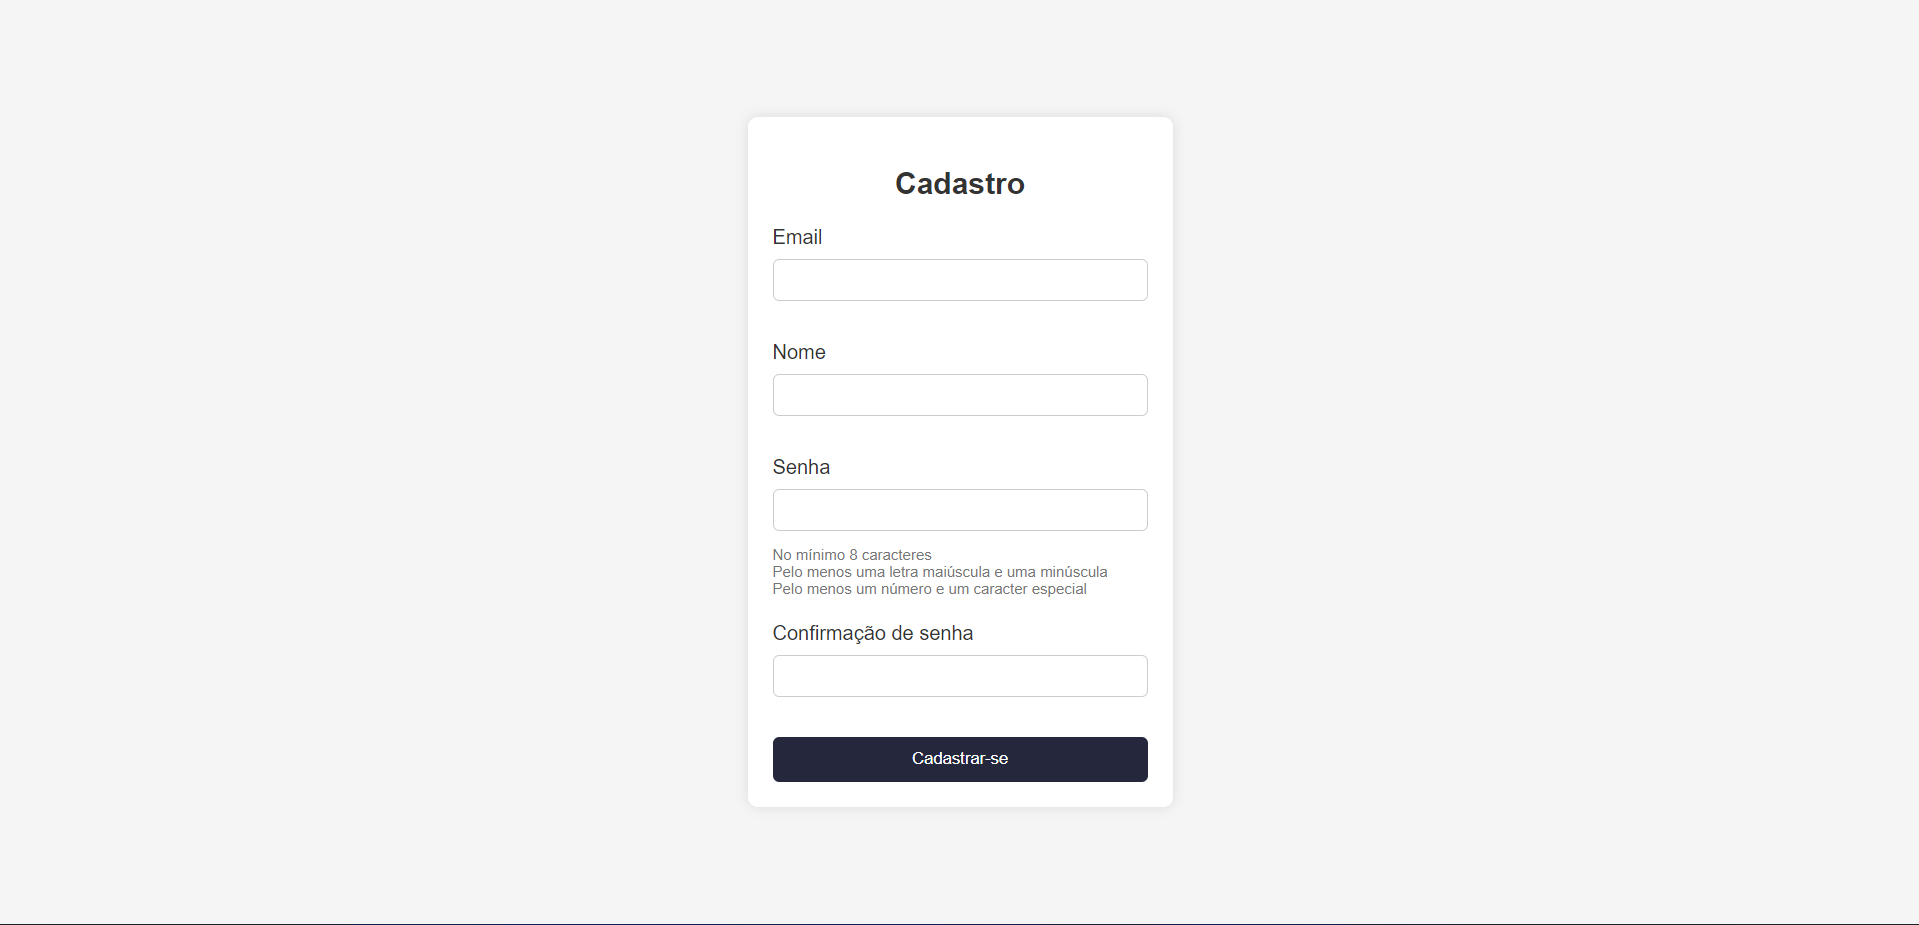
\includegraphics[scale=0.38]{images/cadasto.png}
	\end{center}
	\fonte{Elaborado pelo Autor (2023)}
\end{figure}

A primeira visão do usuário ao entrar no aplicativo está apresentada na \autoref{fig:app-userpage}, nesta página é possível visualizar todos os módulos disponíveis, para este protótipo apenas o “Localizador de Resíduos”.

\begin{figure}[H]
	\caption{\label{fig:app-userpage} Página do usuário}
	\begin{center}
		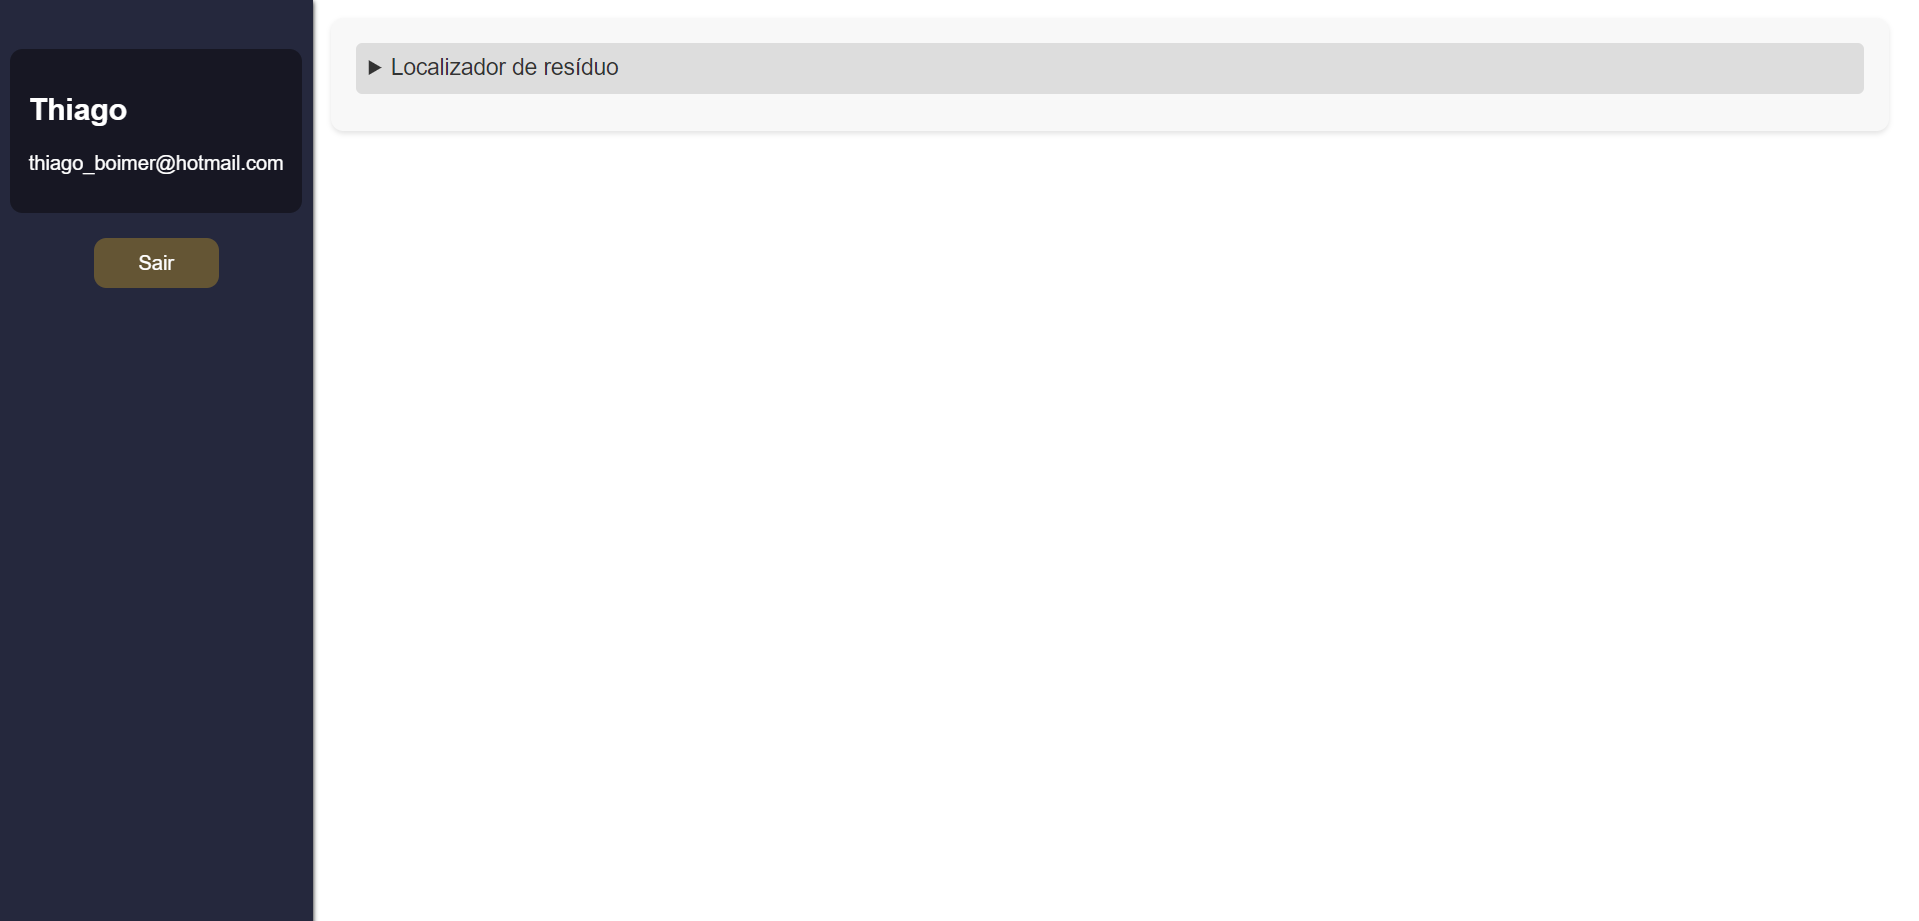
\includegraphics[scale=0.38]{images/user-page.png}
	\end{center}
	\fonte{Elaborado pelo Autor (2023)}
\end{figure}

Ao expandir o módulo, podemos observar na \autoref{fig:app-localizador} uma breve descrição e a estruturação dos campos necessários para a combinação, sendo eles: Capítulo, Subcapítulo e Código do \gls{IBAMA}, o Município e a quantidade de resíduo necessária.

\begin{figure}[H]
	\caption{\label{fig:app-localizador} Módulo de localização de resíduos}
	\begin{center}
		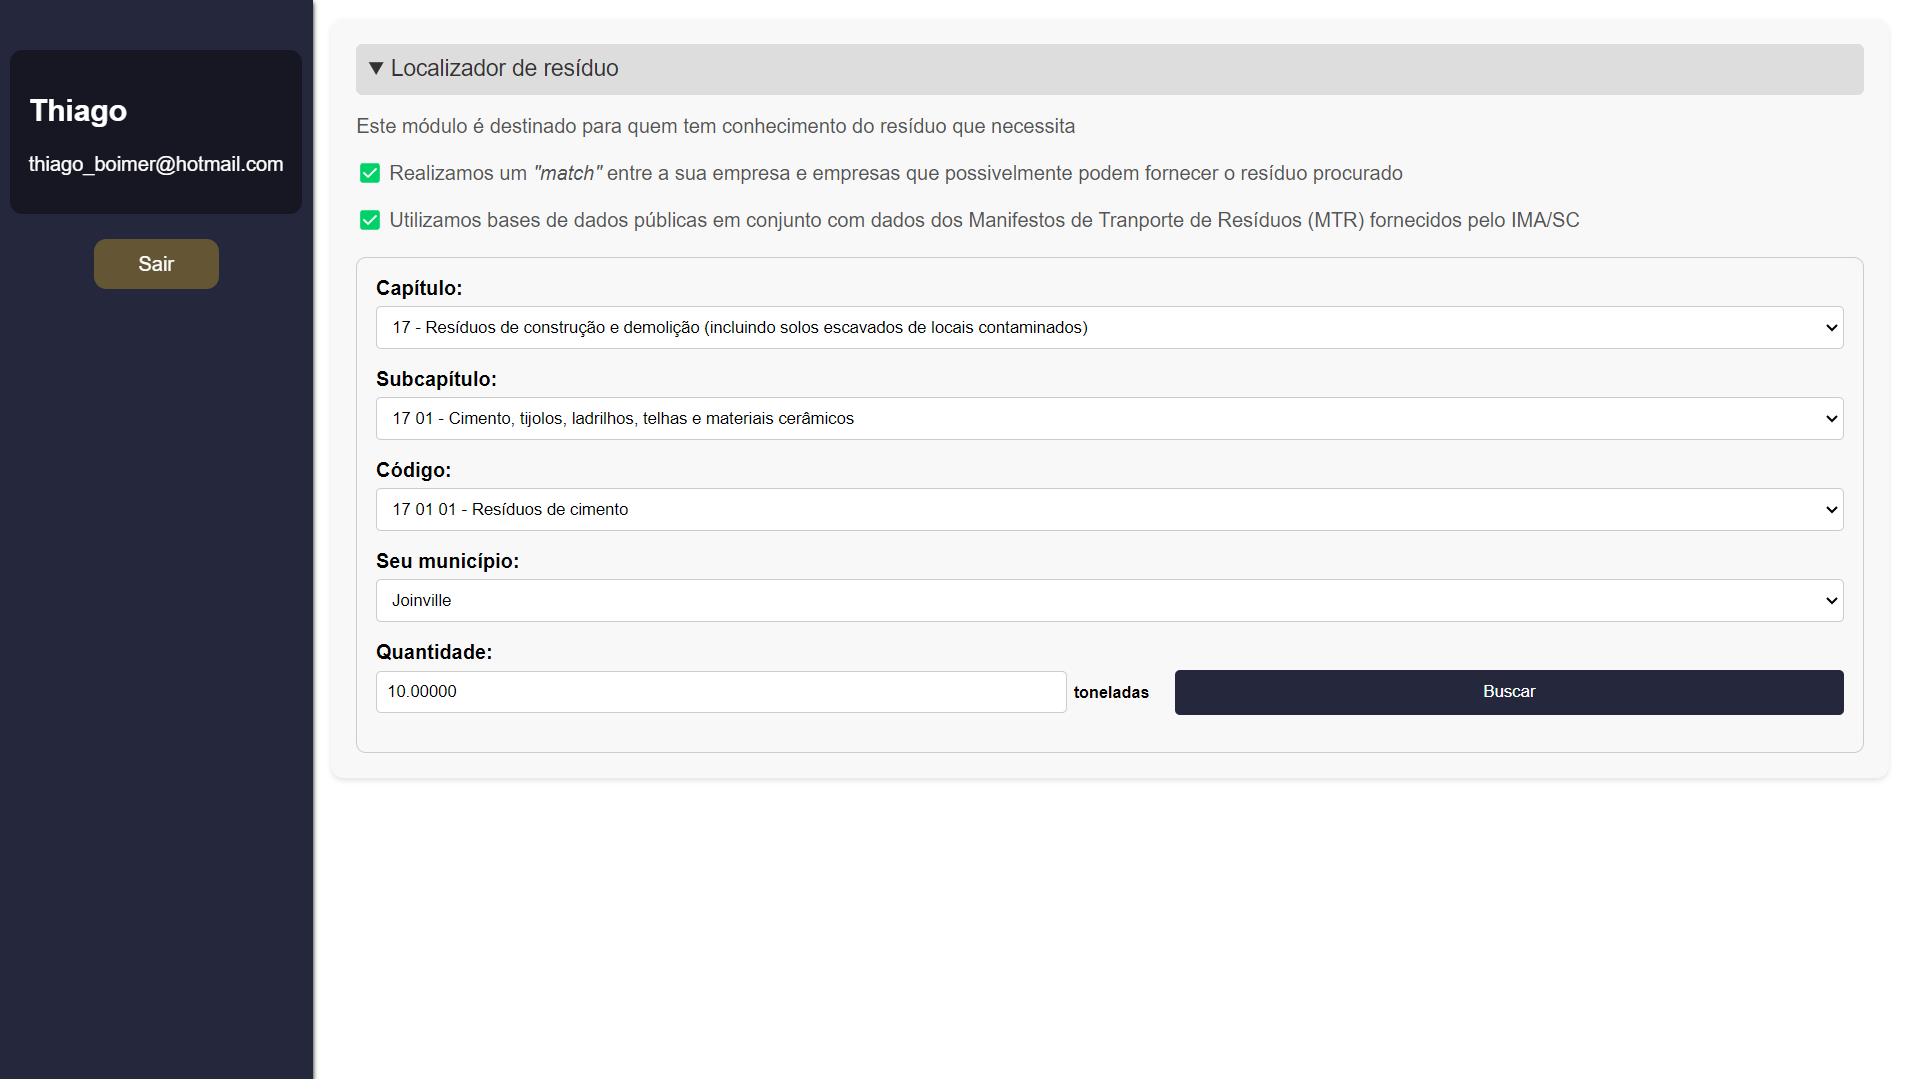
\includegraphics[scale=0.38]{images/localizador-residuo.png}
	\end{center}
	\fonte{Elaborado pelo Autor (2023)}
\end{figure}

Ao finalizar o preenchimento e clicar em buscar, o usuário recebe os resultados em forma de lista decrescente de empresas de acordo com o respectivo score. Cada empresa contém informações relevantes ao match registradas em uma caixa. As caixas possuem cores para melhorar a visualização do score, o “Verde” representando um candidato recomendado (score de 5 a 10), “Amarelo” parcialmente recomendado (score de 1 a 4) e “Vermelho” pouco ou não recomendado.

\begin{figure}[H]
	\caption{\label{fig:app-resultado} Painel de resultados}
	\begin{center}
		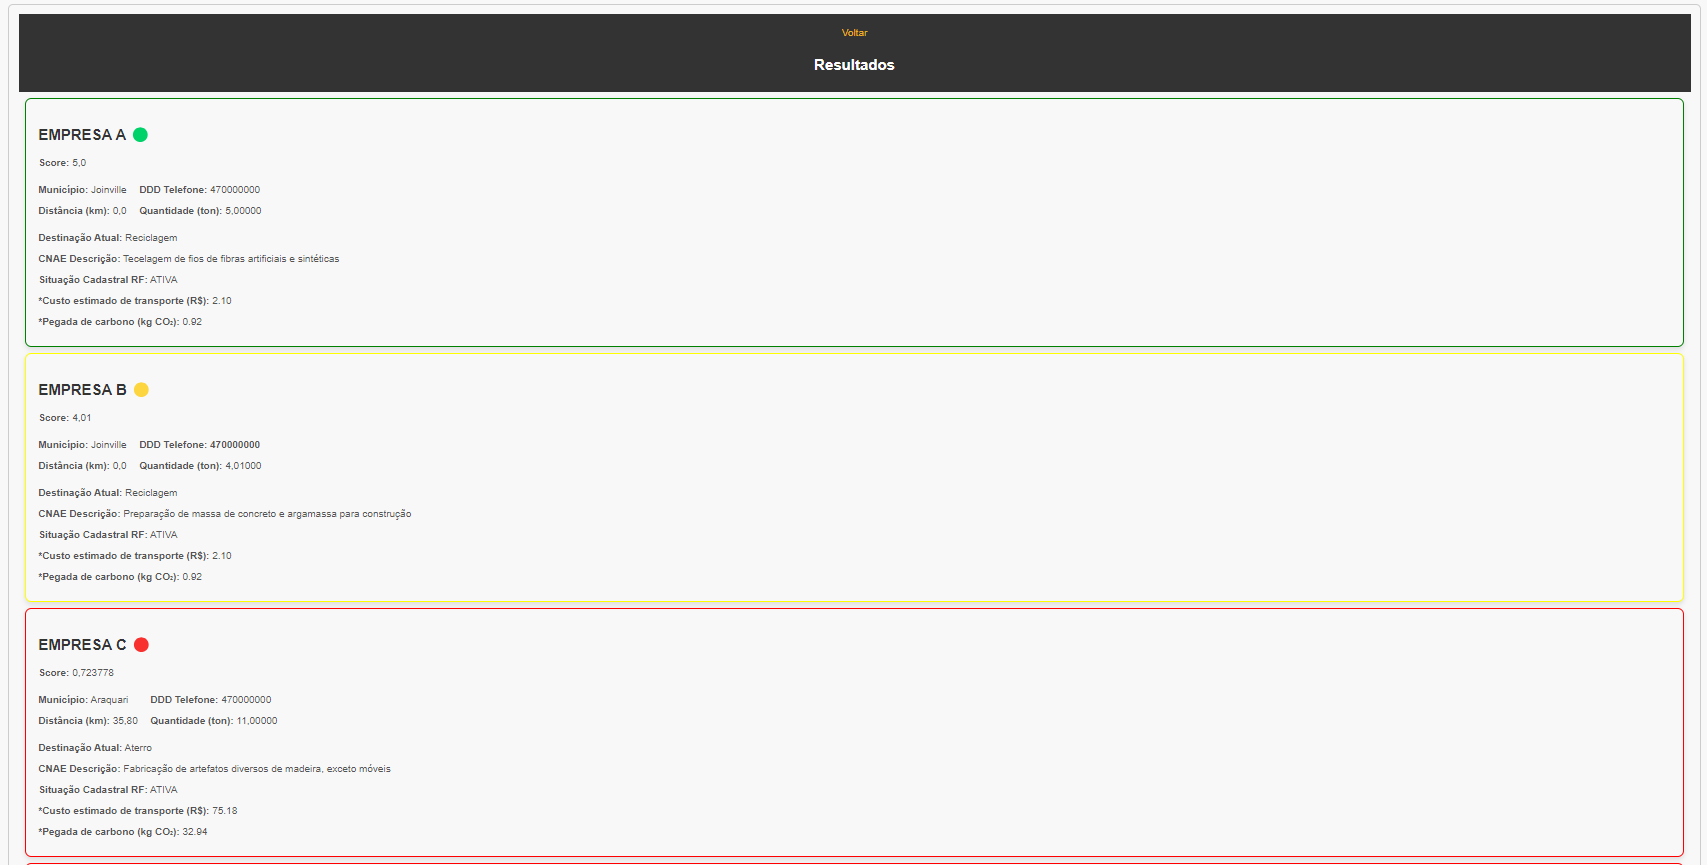
\includegraphics[scale=0.44]{images/localizador-residuo-resultado.png}
	\end{center}
	\fonte{Elaborado pelo Autor (2023)}
\end{figure}


% ----------------------------------------------------------
\subsection{Limitações}
% ----------------------------------------------------------

Ainda que esteja funcional, o protótipo possui muitas limitações, algumas citadas abaixo:

\begin{itemize} 
	\item A localização das empresas foi considerada estar no centroide do município, não devido à falta do endereço completo, mas aos recursos disponíveis no \gls{IBGE}, no ano em que se escreve esse trabalho, apenas a malha de municípios está disponível. Em vista disso, a distância de empresas na mesma cidade do usuário será 0, e o score terá valor máximo se a empresa possuir 80\% da quantidade solicitada;
  \item A distância entre empresas é calculada a partir da melhor rota, contudo o serviço utilizado é gratuito e por isso possui limites de uso, logo se houverem muitas solicitações, o aplicativo deixará de exibir resultados ou simplesmente irá travar;
  \item Não há paginação nos resultados, logo se houverem 1000 combinações, todas serão exibidas, o que pode causar lentidão no navegador do usuário;
  \item O score visual não é dinâmico, de modo que uma busca que apresente apenas valores abaixo de 1, por exemplo, sejam considerados não recomendados, quando na verdade, deveriam estar em formato decrescente de recomendação;
  \item Os dados de \gls{MTR} compreendem a uma geração de dois anos, logo o dado de quantidade disponível de uma empresa não remete à realidade.
\end{itemize}

% ----------------------------------------------------------
\subsection{Possíveis adições e melhorias}
% ----------------------------------------------------------

Além das propostas do Conceito II, podem-se elencar as seguintes melhorias ao aplicativo em questão:

\begin{itemize} 
	\item Aumentar a precisão da localização. Existem outras formas de alcançar uma maior precisão, por métodos simples e pagos ou mais complexos e gratuitos.
  \item Montar um banco de dados com todas as distâncias das melhores rotas entre cidades de SC, de modo a agilizar a busca e não depender do uso de um serviço externo;
  \item Criar a paginação dos resultados para melhor performance e interface;
  \item Desenvolver um score visual que mude dinamicamente com os resultados exibidos;
  \item Obter dados de \gls{MTR} numa menor granularidade (mensal, pelo menos) e exibir os resultados de acordo;
  \item Incluir o mapa com o trajeto até a empresa, o qual está sendo salvo, porém não exibido;
  \item Adicionar a opção de salvar ou exportar os resultados.
\end{itemize}

% ----------------------------------------------------------
\section{Consolidação dos dados}\label{section:consolida}
% ----------------------------------------------------------

\subsection{Limpeza}

Antes de realizar o cruzamento das diferentes fontes de dados — \gls{MTR}, \gls{IBGE} e \gls{CNPJ} —, na base de \gls{MTR}, foi feita a remoção de registros duplicados e nulos provenientes dos arquivos originais e gerados durantes extração dos relatórios \gls{PDF}. 

Também foi feita a remoção de dados com \gls{CPF} e situação cadastral baixada, pois não se tem publicamente a informação de localização para \gls{CPF}, e se a situação cadastral não está ativa, provavelmente a empresa não está em funcionamento. Além disso, durante o cruzamento foi observado que algumas empresas estavam com cadastro vinculado a cidades fora do estado, tais empresas foram removidas. Essas ações previnem que erros sejam multiplicados para as próximas etapas e prejudiquem a análise. A tabela resultante tem a estrutura demonstrada na \autoref{tab:Tab_demo1}.

\setcounter{table}{0}

\begin{table}[htb]
    \ABNTEXfontereduzida
    \centering
    \caption{Amostra da estrutura de dados pós limpeza. \label{tab:Tab_demo1}}
    % \resizebox{\textwidth}{!}{
    \begin{tabular}{@{}lllll@{}}
        \toprule
        \textbf{Razão Social} & \textbf{CNPJ} & \textbf{Código do Resíduo} & \textbf{Destinação} & \textbf{Quantidade (\ensuremath{t})} \\ \midrule
        Empresa A & CNPJ A & 190805 & Tratamento de Efluentes & 0,00018 \\
        Empresa B & CNPJ B & 170202 & Reciclagem              & 0.00020 \\
        Empresa C & CNPJ C & 200102 & Reciclagem              & 0.00200 \\ \bottomrule
        \end{tabular}
    % }
    \fonte{Elaborado pelo Autor (2023)}
\end{table}

Nos histogramas da \autoref{fig:hist-quant}, podemos observar no gráfico (a) a distribuição da massa de resíduos gerados ao longo de dois anos (2020 a 2021); destacado em vermelho está a faixa de aproximadamente 10 \ensuremath{g} — 1000 \ensuremath{t}, a qual abrange a maior parte das empresas geradoras.
No gráfico (b) o intervalo em (a) está aumentado e dividido em 1000 vezes, destaca-se a faixa de 10 \ensuremath{g} — 1 \ensuremath{t}, e considerando que a massa está dividida no total de dois anos, é provável que durante o ano a geração seja muito pequena, inviabilizando a inserção em etapas de um processo produtivo, então decidiu-se por filtrar quantidades de resíduo inferiores a 500 \ensuremath{kg}.

\begin{figure}[htb]
	\caption{\label{fig:hist-quant} Histograma da geração de resíduos sólidos em SC (2020 e 2021)}
	\begin{center}
		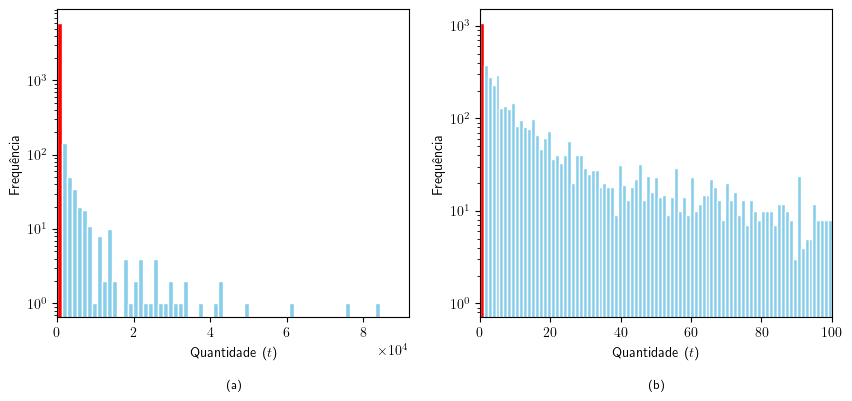
\includegraphics[scale=0.75]{images/hist-quantidade.png}
	\end{center}
	\fonte{Elaborado pelo Autor (2023)}
\end{figure}

\subsection{Cruzamento}

Esta etapa consiste na ligação entre as bases restantes, através dos dados de \gls{CNPJ} podemos identificar a localização da empresa no Portal de Dados Abertos, e com essa informação obtém-se as coordenadas geográficas do município através dos dados do \gls{IBGE}. Dessa forma, temos todas as variáveis necessárias para listar as empresas que podem atuar como fornecedoras da matéria-prima que outra empresa deseja; a tabela final para realizar a conexão entre as empresas está amostrada na \autoref{tab:Tab_demo2}.

\begin{table}[htb]
    \ABNTEXfontereduzida
    \centering
    \caption{Amostra da estrutura de dados pós cruzamento. \label{tab:Tab_demo2} }
    \resizebox{\textwidth}{!}{
    \begin{tabular}{@{}llllllllll@{}}
    \toprule
    \textbf{Razão Social} &
        \textbf{CNPJ} &
        \textbf{CNAE} &
        \textbf{Município} &
        \textbf{Longitude} &
        \textbf{Latitude} &
        \textbf{Código do Resíduo} &
        \textbf{Destinação} &
        \textbf{Quantidade (\ensuremath{t})} \\ \midrule
    Empresa A & CNPJ A & Fabricação de esquadrias de metal & Joinville     & -26.2443 & -48.9514 & 190805 & Tratamento de Efluentes & 0,00018 \\
    Empresa B & CNPJ B & Fundição de ferro e aço           & Criciúma      & -28.7157 & -49.3797 & 170202 & Reciclagem              & 0.00020 \\
    Empresa C & CNPJ C & Laboratórios clínicos             & Florianópolis & -27.5788 & -48.5091 & 200102 & Reciclagem              & 0.00200 \\ \bottomrule
    \end{tabular}
    }
    \fonte{Elaborado pelo Autor (2023)}
\end{table}


\section{Análise exploratória dos dados}
% ----------------------------------------------------------

No momento em que se escreve esse relatório, não se encontram informações disponíveis publicamente sobre os \gls{MTR}s, logo considera-se válido realizar uma análise para se obter um panorama geral da Geração e Destinação de \gls{RSI}s em \gls{SC}. 

\subsection{Geração}
% ----------------------------------------------------------

Dentre os 877 resíduos da classificação do \gls{IBAMA}, de acordo com os relatórios de \gls{MTR}, 135 estão em circulação no estado. Na \autoref{fig:cap-quant}, mostra-se a distribuição da quantidade \ensuremath{t} de geração de resíduos sólidos por capítulo, na \autoref{tab:tab-cap-ibama} do Anexo A — Classificação de Resíduos Sólidos por Capítulos do IBAMA, tem-se a referência para a descrição dos Capítulos.

\begin{figure}[htb]
	\caption{\label{fig:cap-quant} Geração de resíduos sólidos classificados por capítulo em SC (2020 e 2021)}
	\begin{center}
		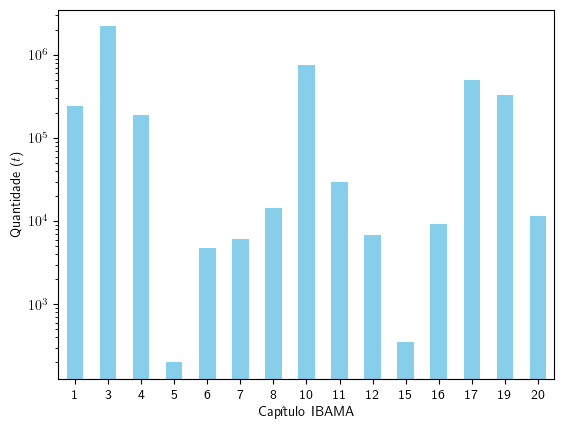
\includegraphics[scale=0.75]{images/cap-quantidade.png}
	\end{center}
	\fonte{Elaborado pelo Autor (2023)}
\end{figure}

Os capítulos com maiores gerações são os 3, 10, 17, 19, 1 e 4, em ordem decrescente de quantidade, correspondendo acerca de 90\% da massa de resíduos gerada em dois anos. Na \autoref{tab:top-res} estão representados os resíduos com maior geração por capítulo.


\newcolumntype{M}[1]{>{\centering\arraybackslash}m{#1}}

\begin{landscape}
    \topskip0pt
    \vspace*{\fill}
\begin{table}[htb]
    \ABNTEXfontereduzida
    \centering
    \caption{Resíduos sólidos predominantes por capítulo \label{tab:top-res} }
    \begin{tabular}{@{}c M{8cm} M{2cm} M{8cm} M{3cm}@{}}
        \toprule
        \multicolumn{1}{l}{\textbf{Capítulo}} &
          \textbf{Descrição Capítulo} &
          \textbf{Código Resíduo} &
          \textbf{Descrição Resíduo} &
          \textbf{Qtd (\ensuremath{t}) $10{^3}$} \\ \midrule
          3 &
          Resíduos do processamento de madeira e da fabricação de painéis, mobiliário, papel e celulose &
          030308 &
          Resíduos da triagem de papel e papelão destinado a reciclagem &
          513 \\ \hline
        1 &
          Resíduos da prospecção e exploração de minas e pedreiras, bem como de tratamentos físicos e químicos das matérias extraídas &
          010409 &
          Areias e argilas &
          226 \\ \hline
        17 &
          Resíduos de construção e demolição (incluindo solos escavados de locais contaminados) &
          170504 &
          Solos e rochas não abrangidos em 17 05 03 &
          196 \\ \hline
        10 &
          Resíduos de processos térmicos &
          100101 &
          Cinzas, escórias e poeiras de caldeiras (excluída as poeiras   de caldeiras abrangidas em 10 01 04) &
          152 \\ \hline

        19 &
          Resíduos de instalações de gestão de resíduos, de estações de tratamento de águas  residuais e da preparação de   água para consumo humano e água para consumo industrial &
          190805 &
          Lodos do tratamento de efluentes urbanos &
          139 \\ \hline
        4 &
          Resíduos da indústria do couro e produtos de couro e da indústria têxtil &
          040215 &
          Resíduos dos acabamentos não abrangidos em 04 02 14 &
          86
        \end{tabular}
    \fonte{Elaborado pelo Autor (2023)}
    \end{table}
    \vspace*{\fill}
\end{landscape}

Na \autoref{fig:sc-geracao}, pode-se ter uma visão macro da geração de resíduos por município em \gls{SC}. Por questões estéticas nem todos nomes estão exibidos, porém é possível acessar o mapa de forma interativa no site: \url{https://residuose.tech/mapa-geracao-sc}. A \autoref{tab:sc-geracao} lista os municípios com geração acima de 50 mil toneladas. 

É notável o destaque para o município de Joinville, com 5\% da geração de resíduos sólidos do estado, sendo 65\% dos resíduos: 170504 - Solos e rochas não abrangidos em 17 05 03 \footnote{17 05 03 - (*) Solos e rochas contendo outras substâncias perigosas}. (167 mil \ensuremath{t}),  010409 - Areias e argilas (118 mil \ensuremath{t}), 100903 - Escórias do forno (88 mil \ensuremath{t}).


\begin{figure}[htb]
	\caption{\label{fig:sc-geracao} Mapa da geração de resíduos sólidos por município}
	\begin{center}
		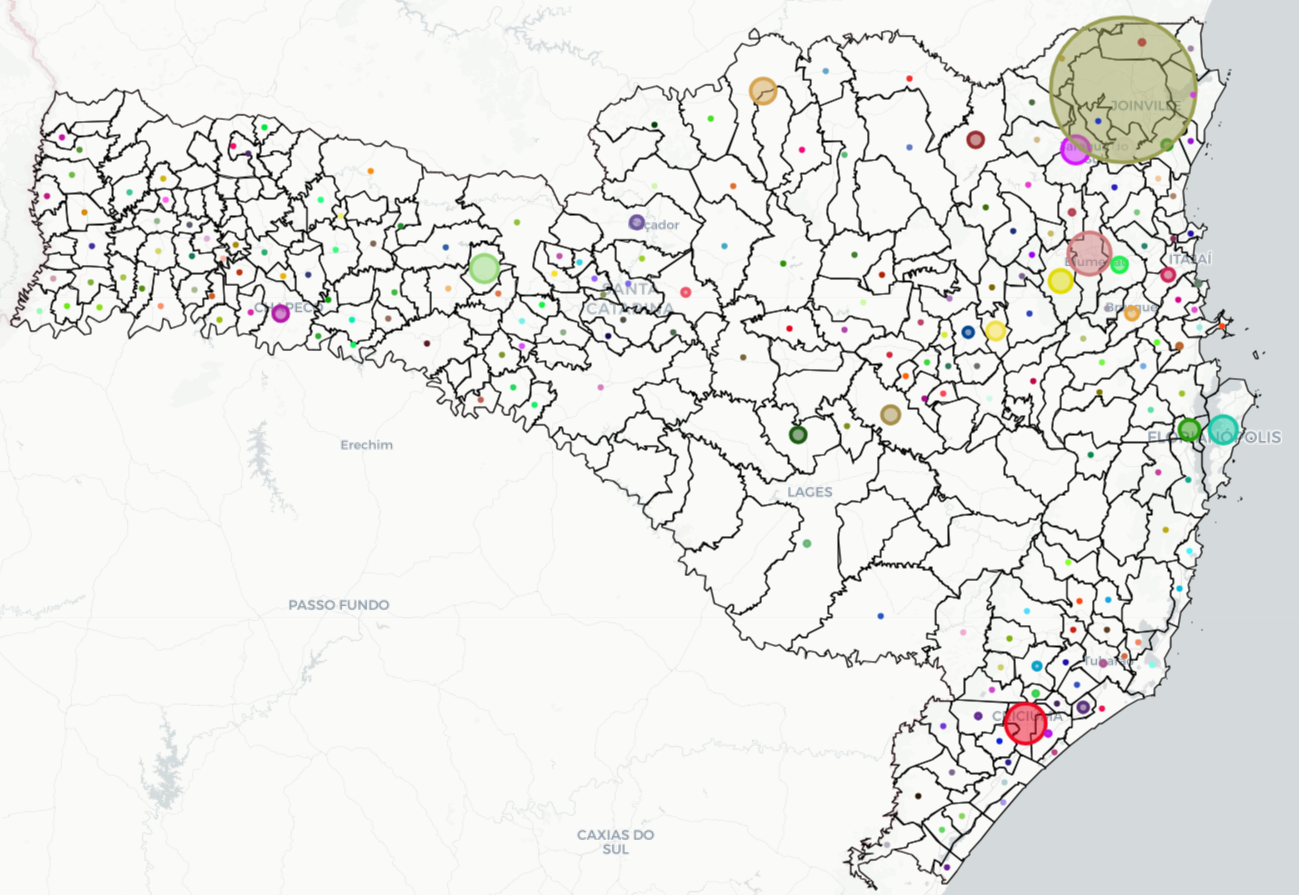
\includegraphics[scale=0.47]{images/sc-geracao.png}
	\end{center}
	\fonte{Elaborado pelo Autor (2023)}
\end{figure}


\begin{table}[htb]
    \ABNTEXfontereduzida
    \centering
    \caption{Geração de resíduos sólidos superior a 50 mil \ensuremath{t} por município  \label{tab:sc-geracao} }
    \begin{tabular}{@{}ll@{}}
    \toprule
    \textbf{Município} & \textbf{Quantidade (\ensuremath{t}) $10{^3}$} \\ \midrule
    Joinville          & 581,41                                        \\
    Blumenau           & 165,89                                        \\
    Criciúma           & 158,95                                        \\
    Jaraguá do Sul     & 114,99                                        \\
    Florianópolis      & 111,45                                        \\
    Vargem Bonita      & 106,61                                        \\
    Canoinhas          & 99,73                                         \\
    Indaial            & 91,13                                         \\
    São José           & 79,10                                         \\
    Guaramirim         & 77,14                                         \\
    Lontras            & 66,93                                         \\
    Otacílio Costa     & 66,57                                         \\
    Rio Negrinho       & 63,10                                         \\
    Chapecó            & 61,98                                         \\
    Gaspar             & 61,19                                         \\
    Correia Pinto      & 58,74                                         \\
    Itajaí             & 52,52                                         \\
    Brusque            & 51,43                                         \\ \bottomrule
    \end{tabular}
    \fonte{Elaborado pelo Autor (2023)}
    \end{table}

\pagebreak
% ----------------------------------------------------------
\subsection{Destinação}
% ----------------------------------------------------------

Com base nos dados de geração, uma vez que o capítulo 03 (Resíduos do processamento de madeira e da fabricação de painéis, mobiliário, papel e celulose) é o predominante no estado, espera-se que a destinação mais praticada seja a de Reciclagem, conforme ilustrado na \autoref{fig:bar-destinacao}, deste valor 45\% é proveniente do cap. 03, 24\% do 17 e 22\% do 10. Para o Aterro, representando 35\% da destinação de resíduos, tem-se 25\% do cap. 10, 17\% do 01 e 19, 16\% do 17 e 13\% do 03.

Considerando que o rastreamento de \gls{MTR}s está sendo efetivo, podemos pontuar que ainda que seja expressiva a destinação tradicional para aterro, \gls{SC} tem explorado as tecnologias alternativas de destinação de resíduos, como podemos ver a utilização de Tratamento Térmico, Uso Agrícola, Coprocessamento e Compostagem. Diante disso, mostra-se um perfil de mercado que, possuindo uma ferramenta que auxilie as indústrias a encontrarem possíveis matérias-primas no meio de tantos resíduos, tem potencial para prover um retorno econômico e ambiental para o estado.

\begin{figure}[htb]
	\caption{\label{fig:bar-destinacao} Destinação de resíduos sólidos por tecnologia}
	\begin{center}
		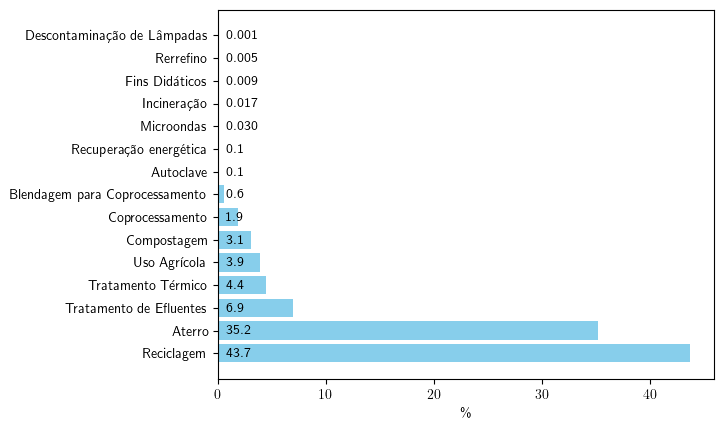
\includegraphics[scale=0.8]{images/bar-destinacao.png}
	\end{center}
	\fonte{Elaborado pelo Autor (2023)}
\end{figure}
